\chapter{Introduction}
\label{chapter-introduction}

% Finite element analysis general description; Motivation example (including image);

Finite Element Analysis (FEA) is the term describing the entire process of modeling the physical system. FEA consists of model generation, meshing, attribute assignment, solution, and post-processing. With the ongoing desire to solve more complex systems with better and better precision, an analysis has to process enormous amount of data in each of its phases. Traditional unstructured file-based representation of the mesh, input parameters, and the results from the solution is the bottleneck of the entire process. It lacks the scalability and complicates the development of the tools for engineers that are either preparing the input to the FEM, or interpreting the output from the FEM.

The solution of large-scale Finite element analysis itself can be parallelized and calculated in reasonable time on high-performance computing clusters. Nevertheless, in the end the results are transfered over network and post-processed on an ordinary personal computer. Another concern is the colaboration and sharing of the model and the results between engineers and researchers. All these limitation of the standard file-based approach lead to re-think the entire process of data management in FEA. The focus of the thesis is mainly on the post-processing of the results, and the way the results are stored, transfered, and visualized. However, the storage format for the results was designed with the whole picture in mind and there is proposed database-centric environment for complete FEA data management.

As an motivation example can serve analysis of reactor vessels in nuclear power plants which is used in the process of prolongation of their service life. The vessels are approximately 40 years old and detailed thermo-hydro-mechanical analysis has to be performed. Usually, two-dimensional axisymmetric or fully three-dimensional models are considered and it means hundreds of thousands degrees of freedom are used. The number of time steps is between 10,000 and 15,000. The output files contain displacements, strain and stress components, temperature, relative humidity (or moisture content) and several internal parameters (e.g. creep strains, damage parameter, etc.) in all time steps. The output files with size in the order of gigabytes are generated. More details can be found in \cite{XXX-1,XXX-2}.

\begin{figure}[H]
\centering
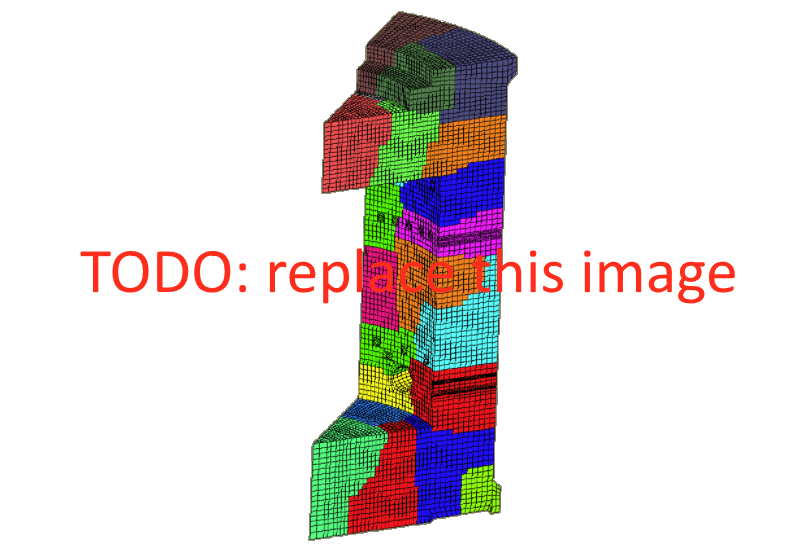
\includegraphics[width=\textwidth]{figures/motivation-example}
\decoRule
\caption[TODO: ]{TODO: Motivation example visualization}
\label{fig:motivation-example}
\end{figure}

%----------------------------------------------------------------------------------------
%	SECTION Concepts
%----------------------------------------------------------------------------------------

\section{Concepts}

% popsat zakladni pojmy se kteryma pracuju, uvod do problemu, ktery se snazim obsahnout; format slovniku - heslo: popis

% vysvetlit, proc pouzivam pojem Multi-mesh (Multigrid byla inspirace)

%----------------------------------------------------------------------------------------
%	SUB-SECTION Finite element analysis
%----------------------------------------------------------------------------------------

\subsection{Finite element analysis}

% nejprve vysvetlit FEM - jak se lisi od FEA

% popsat podrobneji jednotlive faze

\begin{itemize}
    \item Preprocessing / modeller
    \item FEM calculation
    % Finite Element Method (FEM) is .... PD eq, structural analysis, heat transfer, fluid flow, mass transport, and electromagnetic potential. (Wikipedia)
    \item Post-processing of results
\end{itemize}

%----------------------------------------------------------------------------------------
%	SUB-SECTION Storage format
%----------------------------------------------------------------------------------------

\subsection{Storage format} % or Data representation or Data management

% file-based vs. db-based, advantages/disadvantages

% FEA is not an isolated example of this size effect, forcing us to re-think the way we handle application data


%----------------------------------------------------------------------------------------
%	SECTION Challenges
%----------------------------------------------------------------------------------------

\section{Challenges}

% jak reprezentovat takto velke mnozstvi dat
% jak tyto vsechny faze propojit do jednoho systemu
% Jak spravovat projekt/solution, jak propojit model a vysledky, jak umoznit praci vice uzivatelum

% Jak propojit vypocet a vysledky? Zminit multigrid.

% take pouzit styl *heslo* odstavec

%----------------------------------------------------------------------------------------
%	SUB-SECTION Mesh visualization
%----------------------------------------------------------------------------------------

\subsection{Mesh visualization}

% strucne popsat vyzvy vizualizace siti; pak se odkazat na clanek a na appendix

%----------------------------------------------------------------------------------------
%	SUB-SECTION FEM results compression
%----------------------------------------------------------------------------------------

\subsection{FEM results compression}

% vysledku je hodne, je potreba je zmensit; pak se odkazat na 2 clanky a na appendixy
% U approximation clanku jsem se inspiroval multigridem; také zmínit inspiraci mpeg kompresí u aproximace v čase - klíčové snímky

%----------------------------------------------------------------------------------------
%	SECTION Main goal
%----------------------------------------------------------------------------------------

\section{Main goal} % Aims/Goal of the thesis

% zevrubne popsat muj pristup a reseni
% Popsat propojeni systemu, zminit OOFEM-link databazovy model
% Proc jsem se rozhodl vytvorit vlastni format pro ulozeni site a vysledku
% Popsat hlavni charakteristiky tohoto formatu
% odkazat se do appendixu na ukazky formatu? Asi nechat az do pozdejsi kapitoly

% main features for optimization: key time steps (time step span compression), Randomized SVD, Parallelization, Sparse matrix of details, prenasobeni U matice singularnimi cisly, trochu usetrim pamet, mohu pouzit vzorkovani...

